\documentclass[12pt, a4paper]{book}
\begin{document}\label{chap:Best_ML}
\chapter{Model dependent approach}
The results for the network optimizations can be seen in Appendix \ref{chap:network_opt}, where it became apparent that the performance of BDTs is better at scoring a higher significance than NNs, and faster. Because of this and time constraints of this thesis 
we decided to compute the results of the model dependent and model independent search using BDTs only. \\\\
The time has come to test how our networks fare on learning our models. This chapter showcases the results of the method which we called the model dependent approach. This method trains one BDT for each model we have, including all the mass points and simulated samples, 
then we test how well the network has learned the model and create a mass exclusion limit for it.\\
\\To navigate through the process we will take a model as an example, the Dark Higgs Heavy Dark Sector model, and afterwards present the combined exclusion limits for every model. As all of our models had $m_{Z'}=130$ GeV as a lower limit, to reduce computational time 
we decided to make a cut of $m_{ll} >110$ GeV.

\clearpage
\graphicspath{{../../../Plots/}}
\section{Walkthrough of method}\label{sec:Walkthrough}
We conducted a grid search to optimize the BDT and trained the network using 80\% of the SM background samples and 80\% of every different $Z'$ mass sample of the model. Using this approach for this model gave the features in Figure \ref{fig:DH_HDS_feat} as the most important ones. The most important variables here are the ones which we expect 
to be important on a dilepton and MET final state.\\
\begin{figure}[!ht]
	\centering
	\begin{subfigure}[b]{0.7\textwidth}
      \centering
      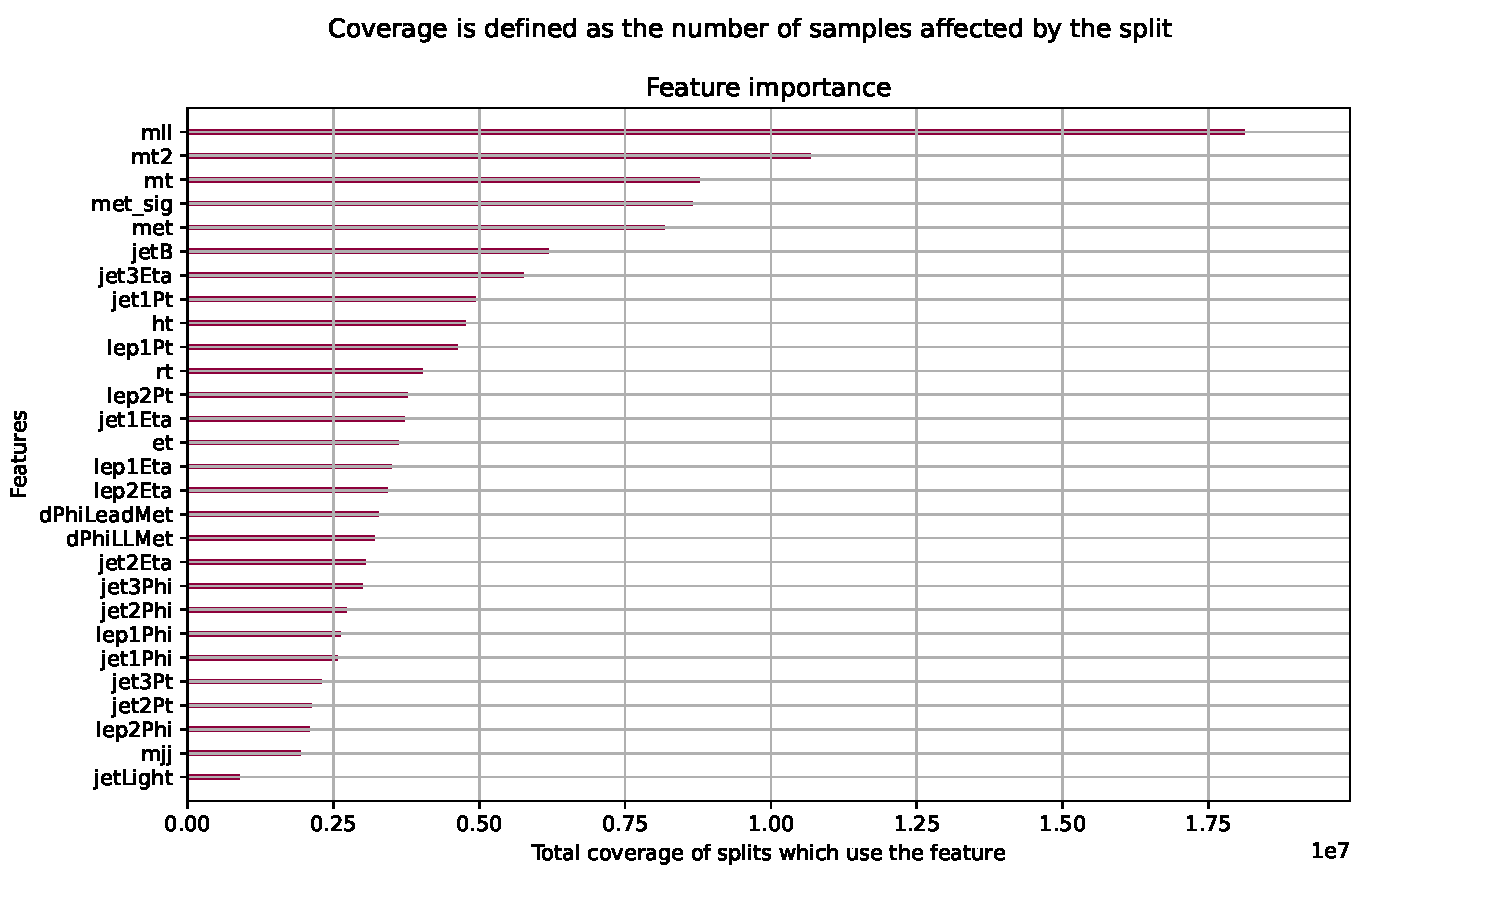
\includegraphics[width=1\textwidth]{XGBoost/DH_HDS/feature_importance/total_cover.pdf}
      \end{subfigure}
      \hfill
      \begin{subfigure}[b]{0.7\textwidth}
         \centering
         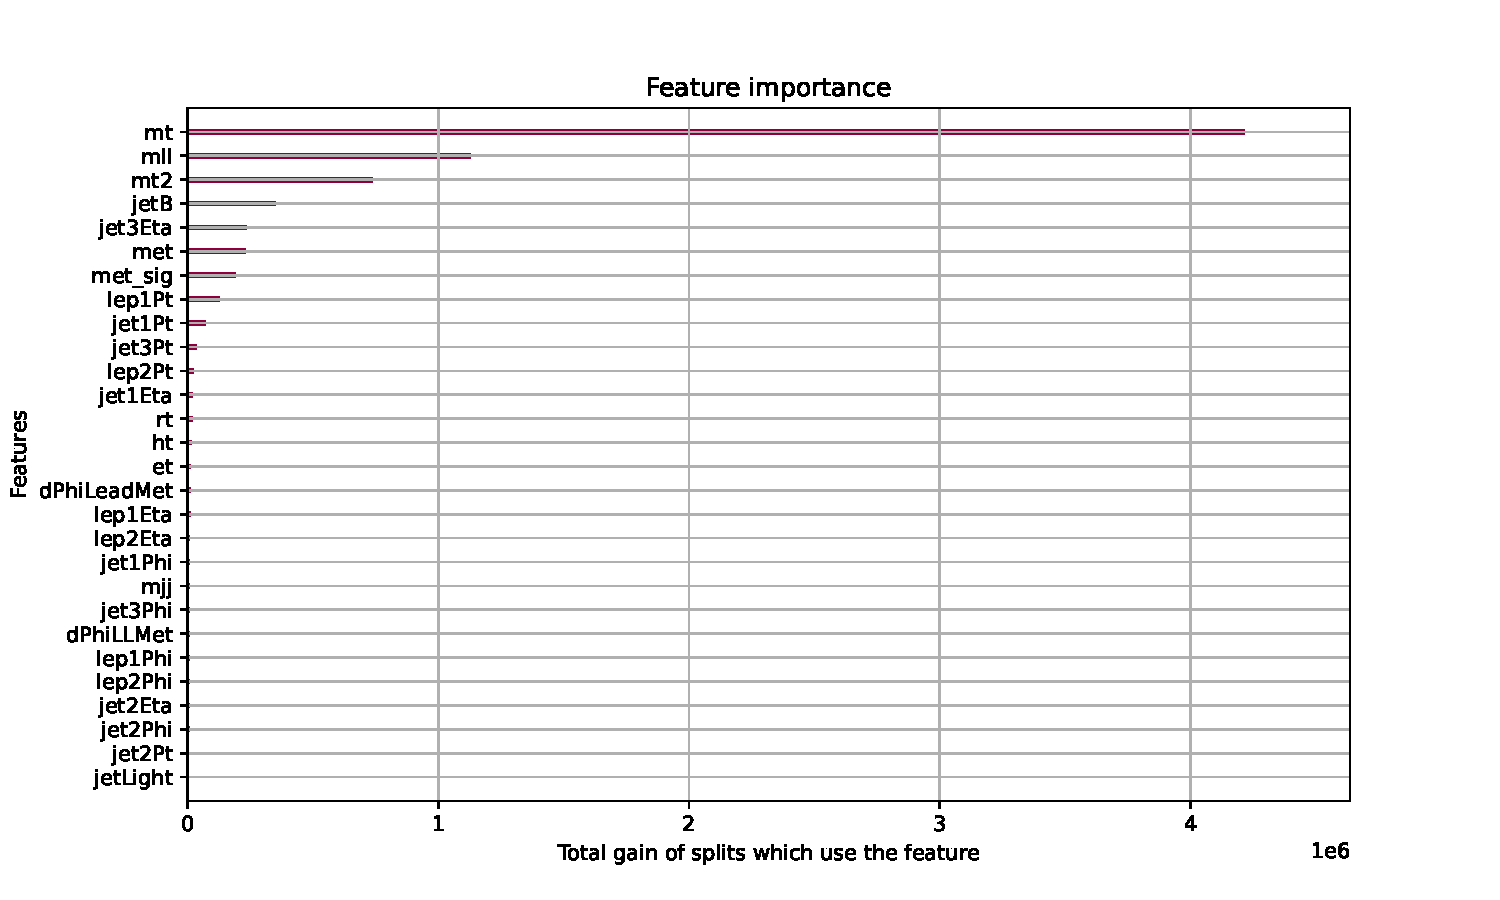
\includegraphics[width=1\textwidth]{XGBoost/DH_HDS/feature_importance/total_gain.pdf}
      \end{subfigure}
      \hfill
      \begin{subfigure}[b]{0.7\textwidth}
         \centering
         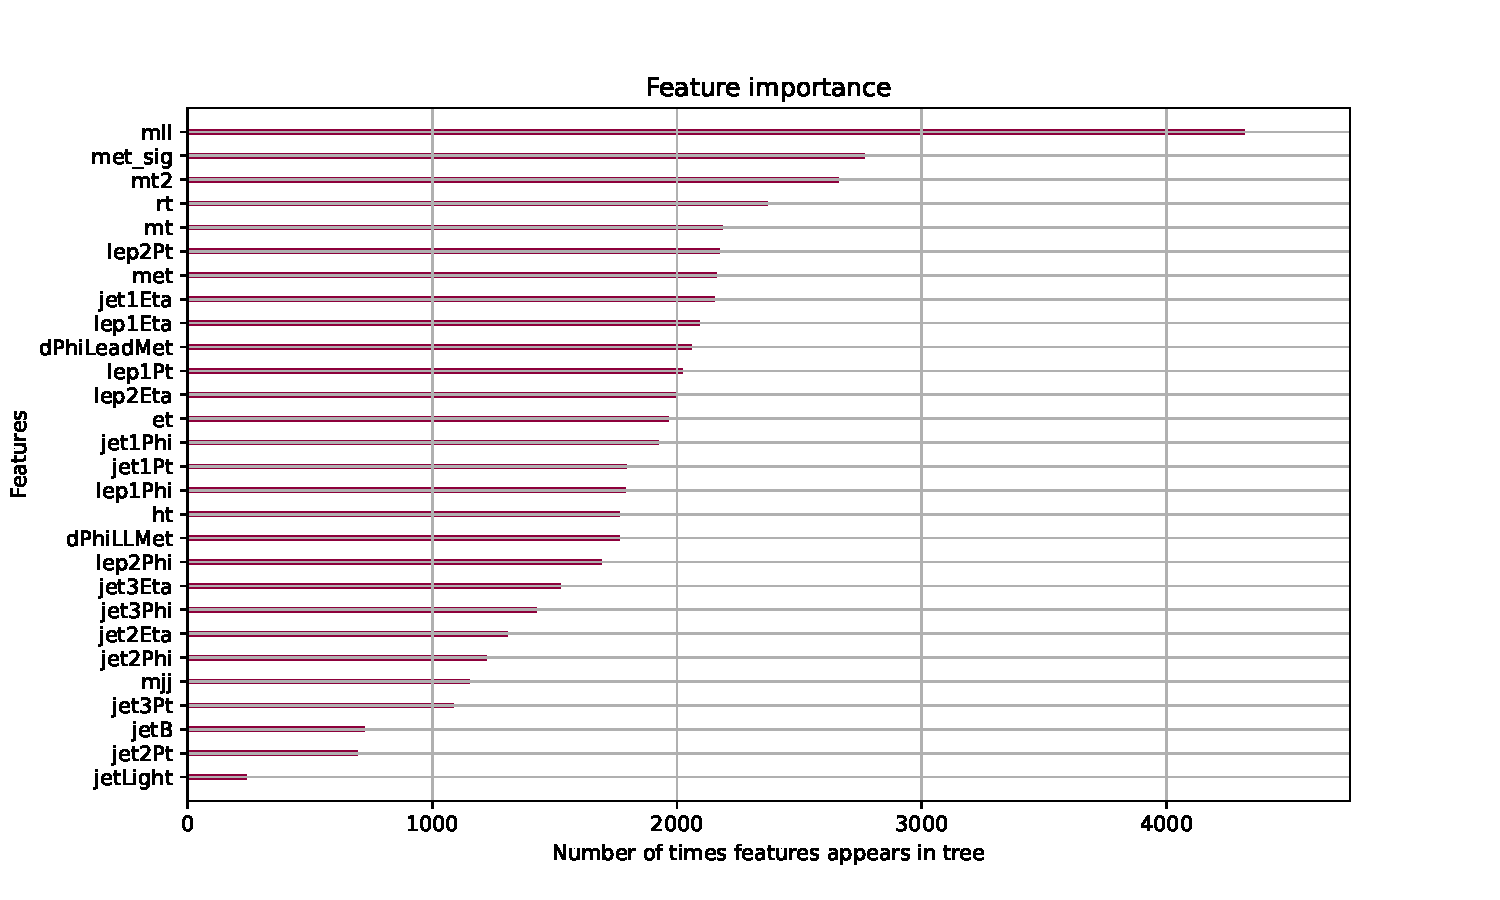
\includegraphics[width=1\textwidth]{XGBoost/DH_HDS/feature_importance/weight.pdf}
      \end{subfigure}
   \caption{Feature importance for network trained on Z' DH HDS}\label{fig:DH_HDS_feat}
\end{figure}
\\To showcase how the network sorts signal from background we can see the validation plots in Figure \ref{fig:DH_HDS_vals} showing all the signal samples which can be seen down to $2\times10^{-3}$ expected events. The reason for this limit is arbitrary and was chosen for aesthetics.\\
\begin{figure}[!ht]
	\centering
	\begin{subfigure}[b]{0.49\textwidth}
      \centering
      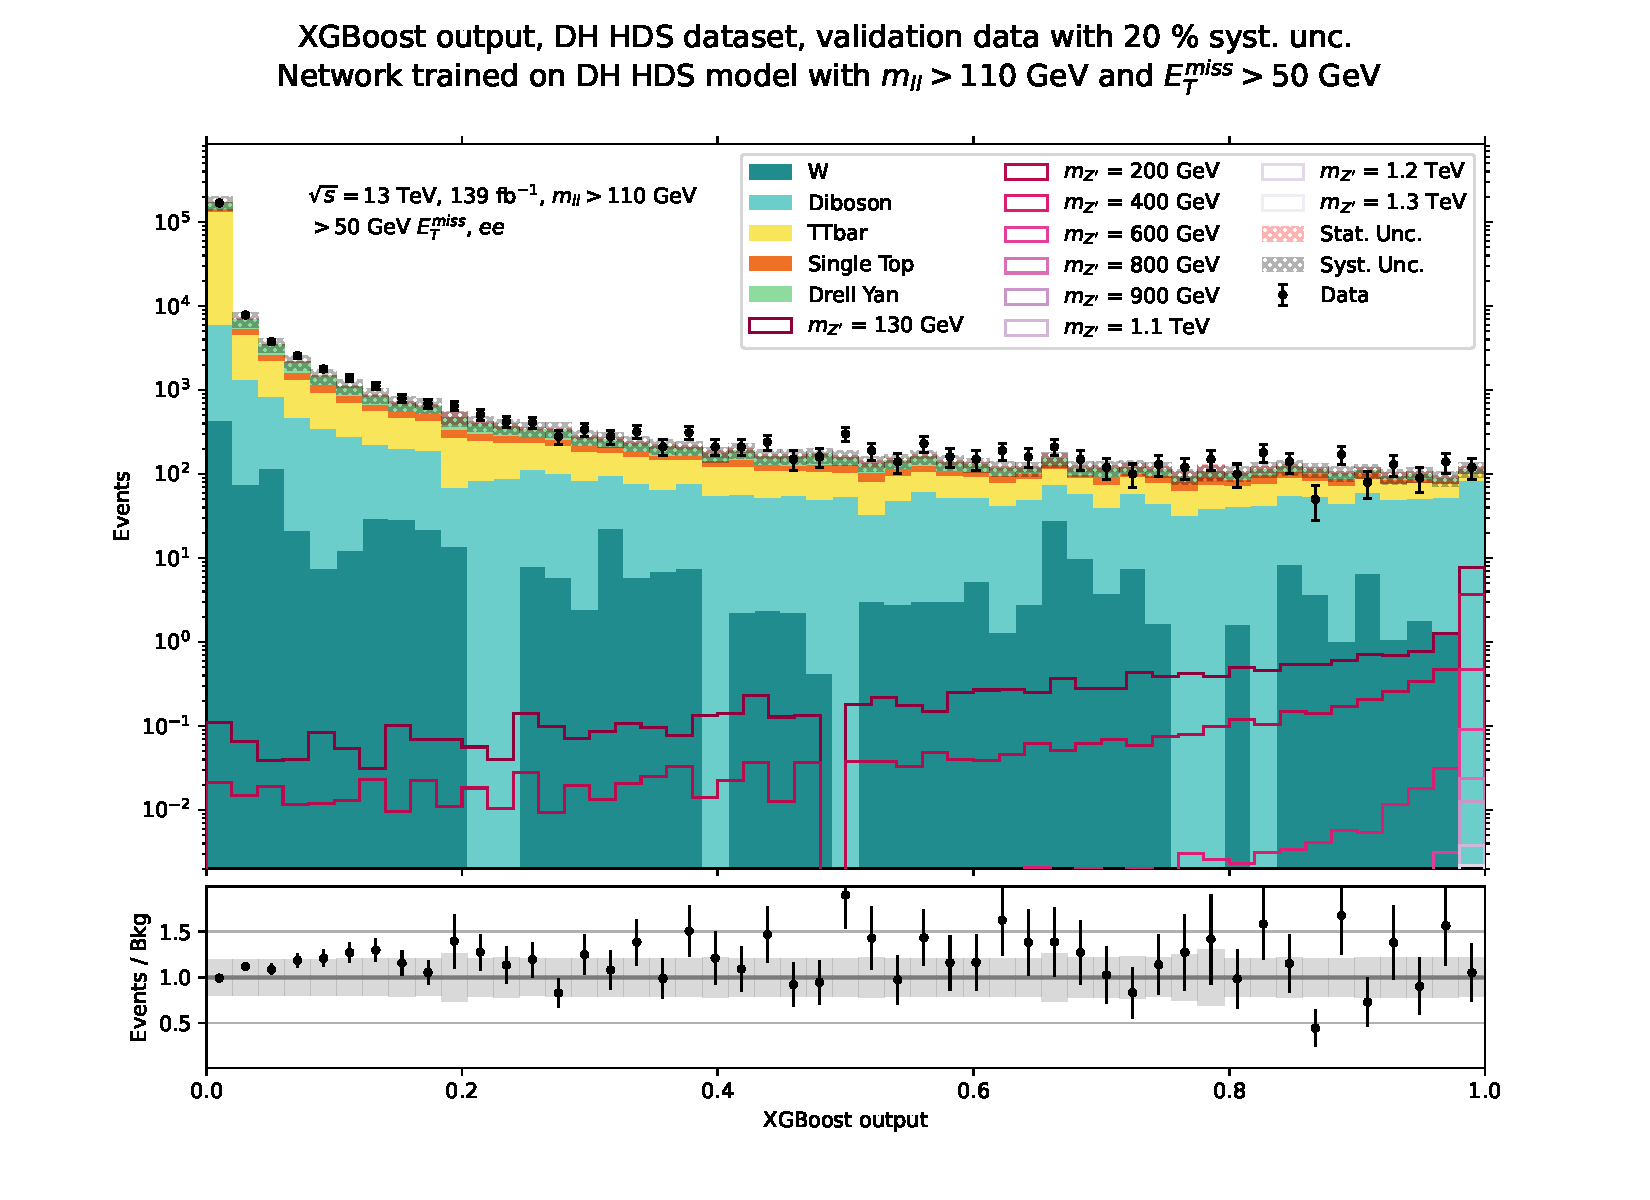
\includegraphics[width=1\textwidth]{XGBoost/DH_HDS/VAL_ee.pdf}
      \end{subfigure}
   \hfill
   \begin{subfigure}[b]{0.49\textwidth}
      \centering
      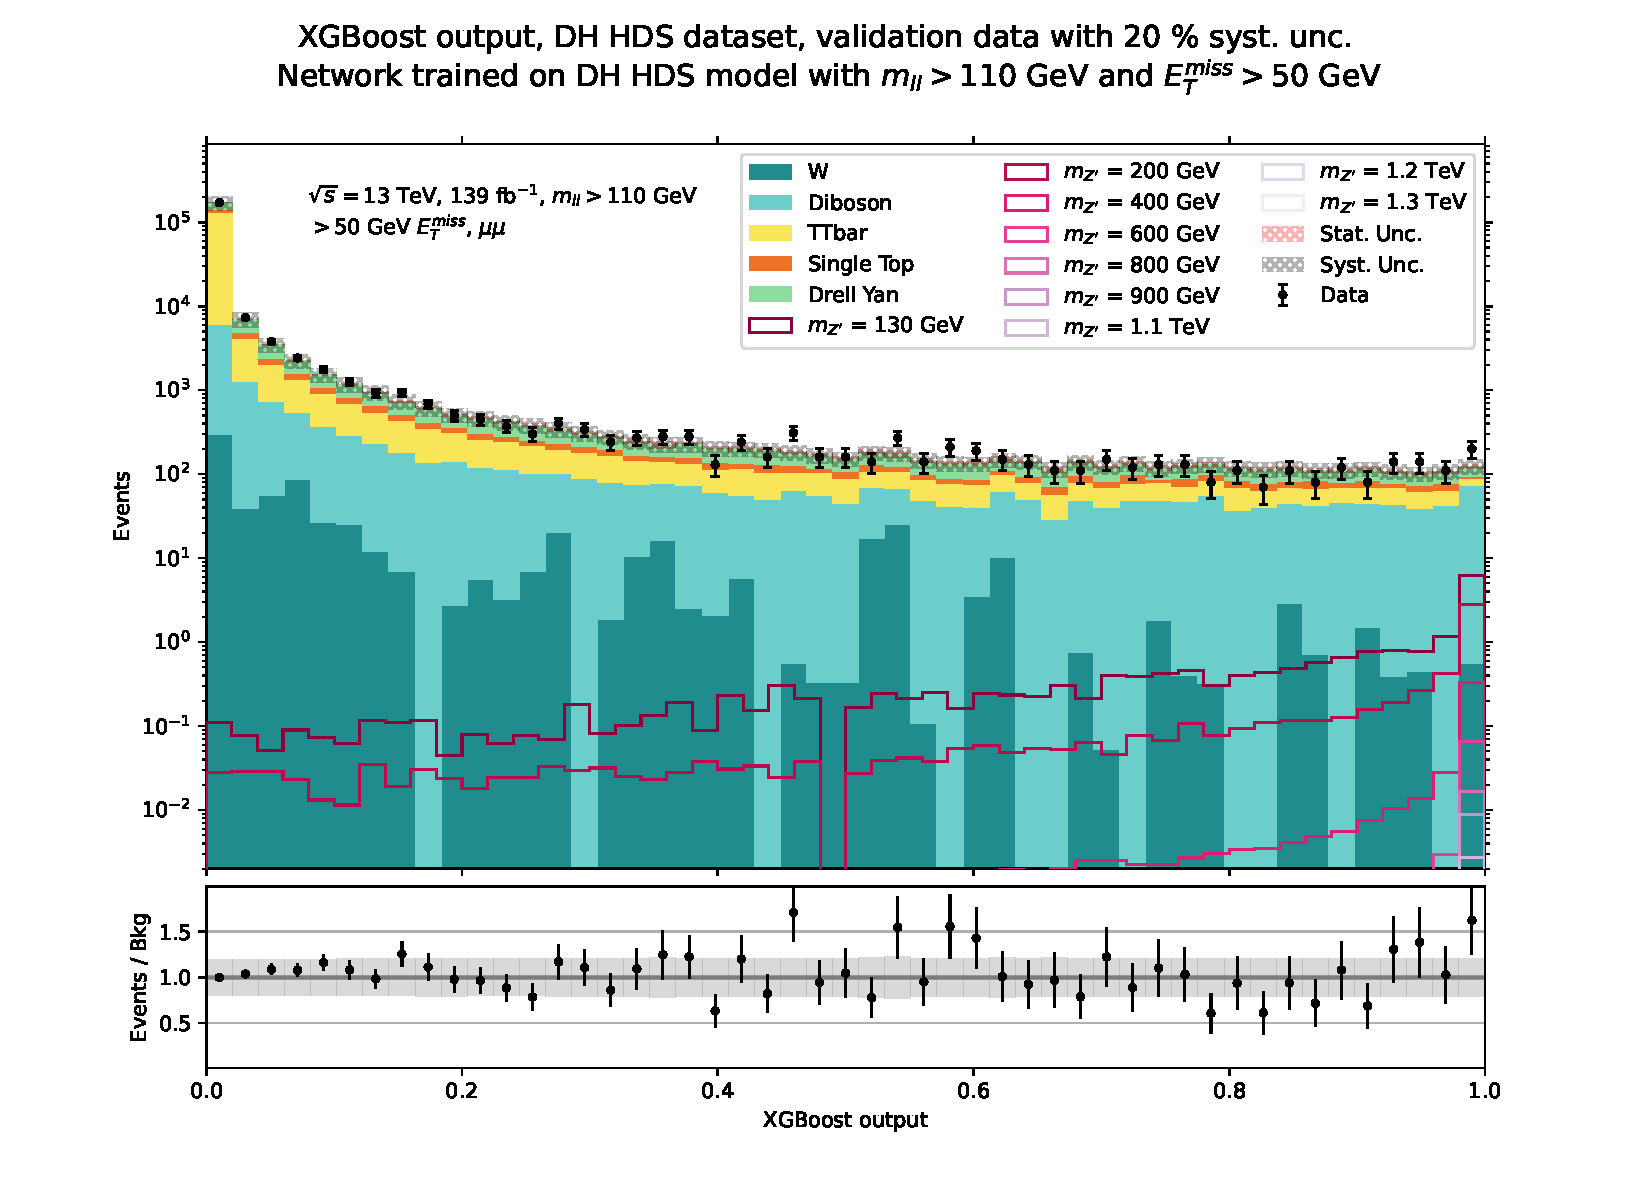
\includegraphics[width=1\textwidth]{XGBoost/DH_HDS/VAL_uu.pdf}
      \end{subfigure}
   \caption{Validation plots for network trained on Z' DH HDS}\label{fig:DH_HDS_vals}
\end{figure}
\\While the validation plot might seem like the network is not doing an impressive job at sorting signal from background, we can actually see how well the network learns the different mass points by looking at the ROC curves for each mass point, this is shown in Figure \ref{fig:DH_HDS_ROCS}. 
Here we see that the network struggles a tiny bit to learn the models with lowest $m_{Z'}$, but the AUC score is still 0.96, meaning that it actually learned to sort the signal from SM background.\\
\begin{figure}[!ht]
	\centering
	\begin{subfigure}[b]{0.49\textwidth}
      \centering
      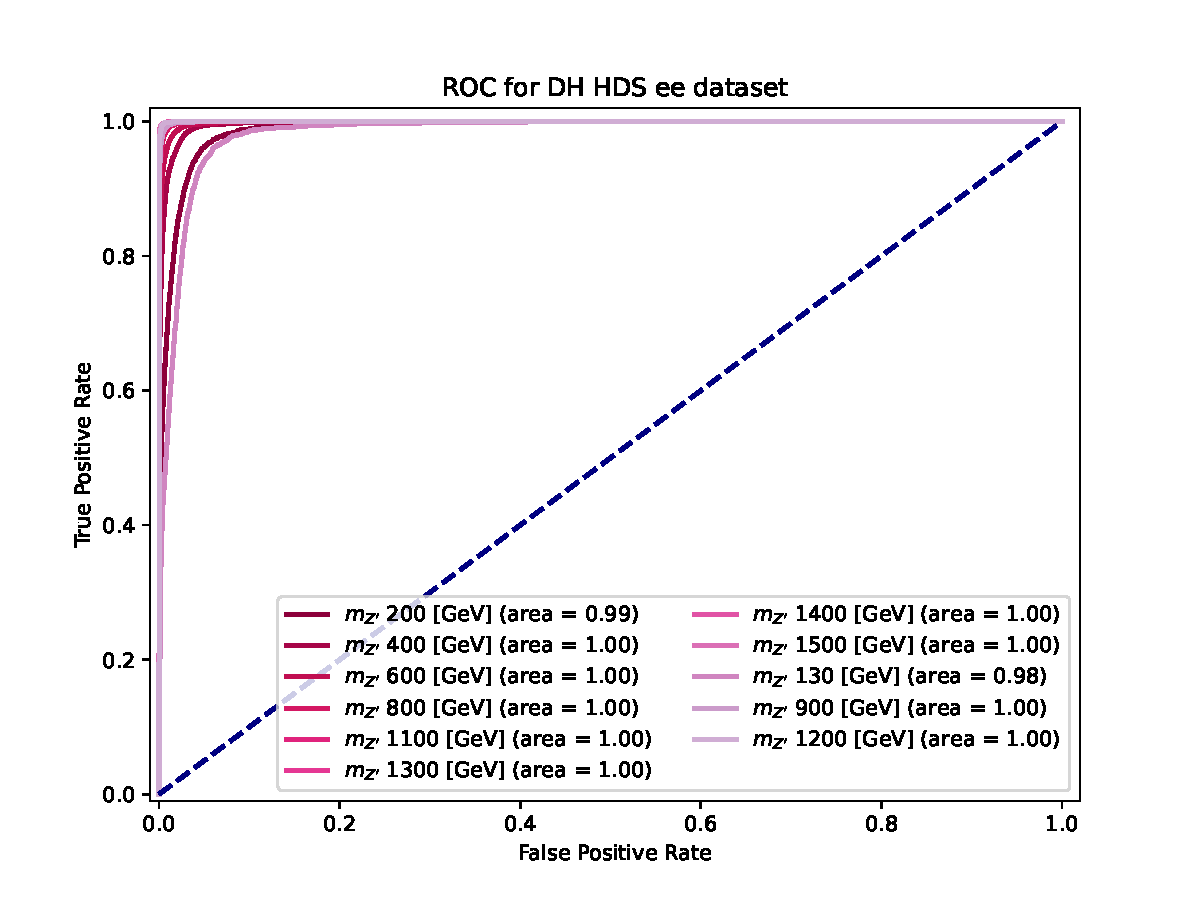
\includegraphics[width=1\textwidth]{XGBoost/DH_HDS/ROC_ee.pdf}
      \end{subfigure}
   \hfill
   \begin{subfigure}[b]{0.49\textwidth}
      \centering
      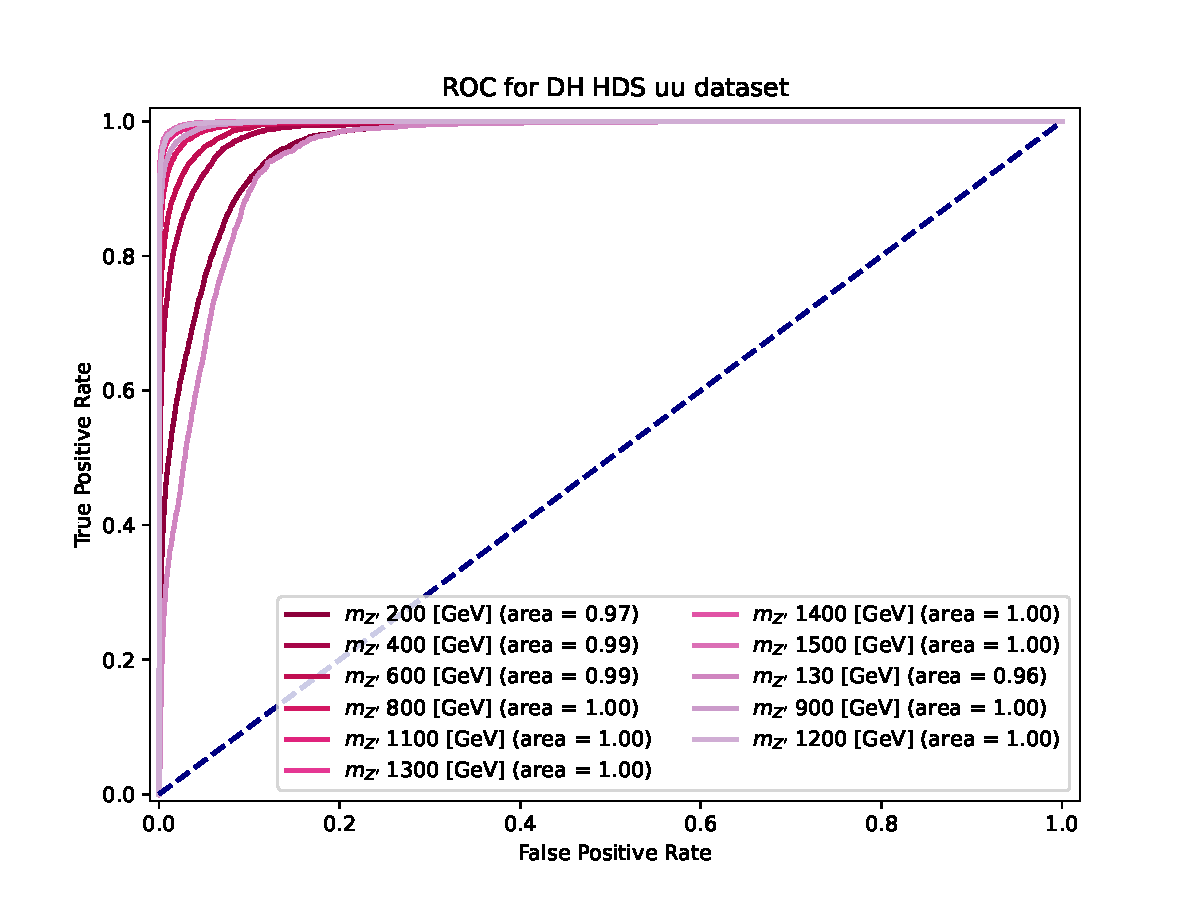
\includegraphics[width=1\textwidth]{XGBoost/DH_HDS/ROC_uu.pdf}
      \end{subfigure}
   \caption{ROC plots for every Z' mass point on network trained on Z' DH HDS}\label{fig:DH_HDS_ROCS}
\end{figure}
\\To define the region we will use to make any exclusions we can choose the validation plot bin that gives us the highest significance, this can be seen in Figure \ref{fig:DH_HDS_exp_sig} for a few mass points (to not drown the plot). From this we see that we get at best an expected significance 
of approximately 0.7$\sigma$ (without uncertainties), even though the network got an AUC score of 0.96 for the mass point on the muon channel. From this we can \textit{conclude} \textbf{Question: is this word way too harsh?} that it is the re-weighting using the cross-section that punishes 
the performance of our networks. This is something that will follow for every result.\\
\begin{figure}[!ht]
	\centering
	\begin{subfigure}[b]{0.49\textwidth}
      \centering
      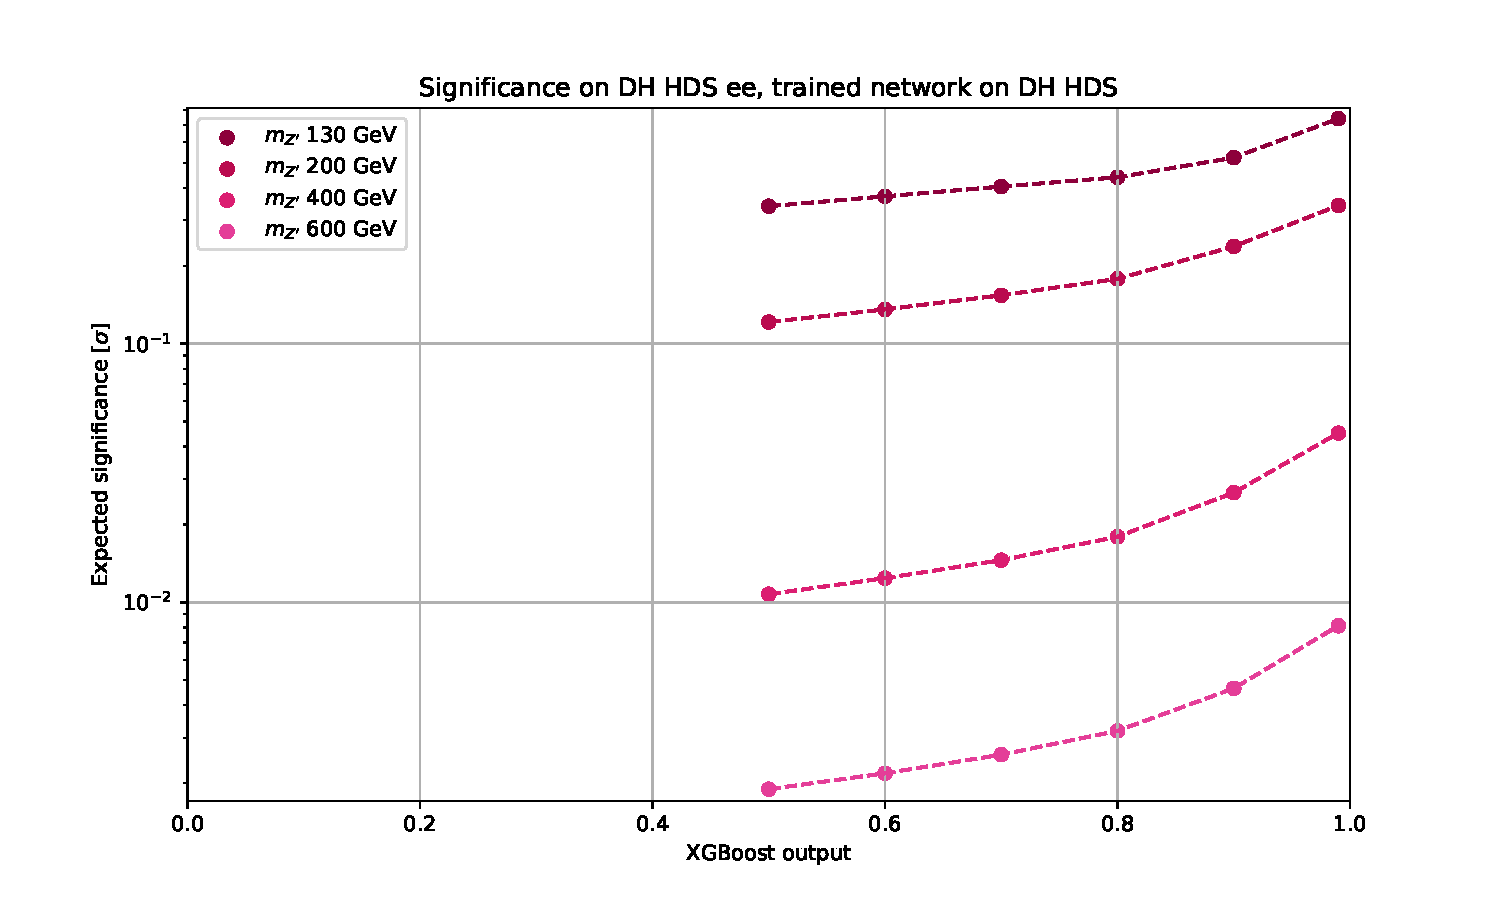
\includegraphics[width=1\textwidth]{XGBoost/DH_HDS/EXP_SIG_ee.pdf}
      \end{subfigure}
   \hfill
   \begin{subfigure}[b]{0.49\textwidth}
      \centering
      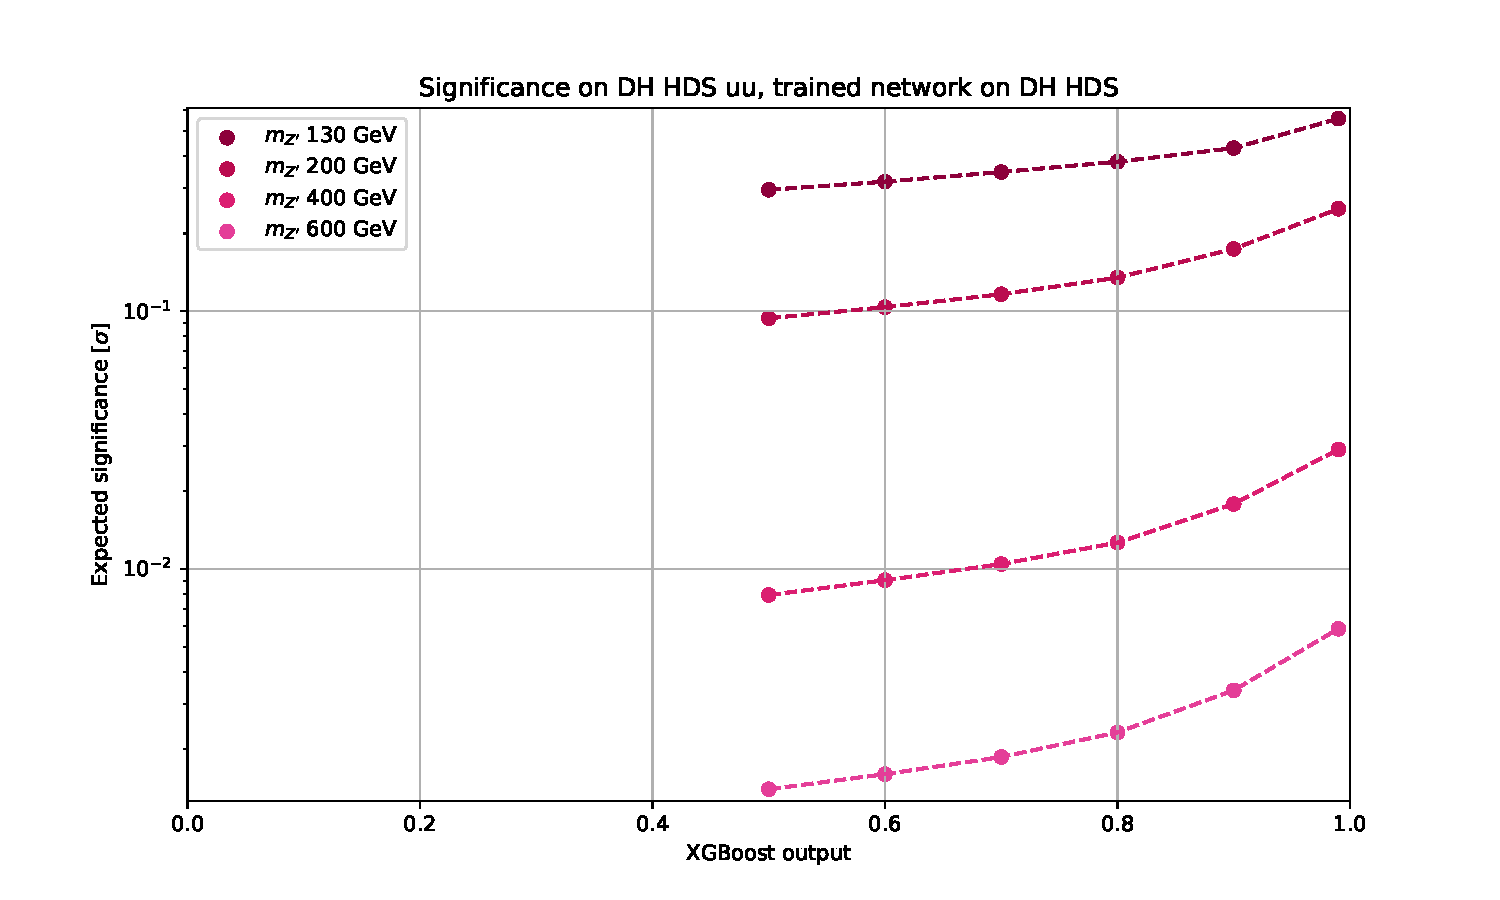
\includegraphics[width=1\textwidth]{XGBoost/DH_HDS/EXP_SIG_uu.pdf}
      \end{subfigure}
   \caption{Expected significance plots for Z' mass points on network trained on Z' DH HDS}\label{fig:DH_HDS_exp_sig}
\end{figure}
\\As the last bin has the greatest significance, we can effectively make a cut based on the BDT score. Counting the number of events on this last bin, as well as their uncertainties we can calculate a mass exclusion for both electron and muon channel. 
Following the method explained in Chapter \ref{sec:stat_anal} using the values in Table \ref{tab:stat_vals_DH_HDS} we can create a mass exclusion for each leptonic channel. The results can be seen in Figure \ref{fig:DH_HDS_exclusion_ee_uu}.
\clearpage
\begin{figure}[!ht]
	\centering
   \begin{subfigure}[b]{0.49\textwidth}
      \centering
      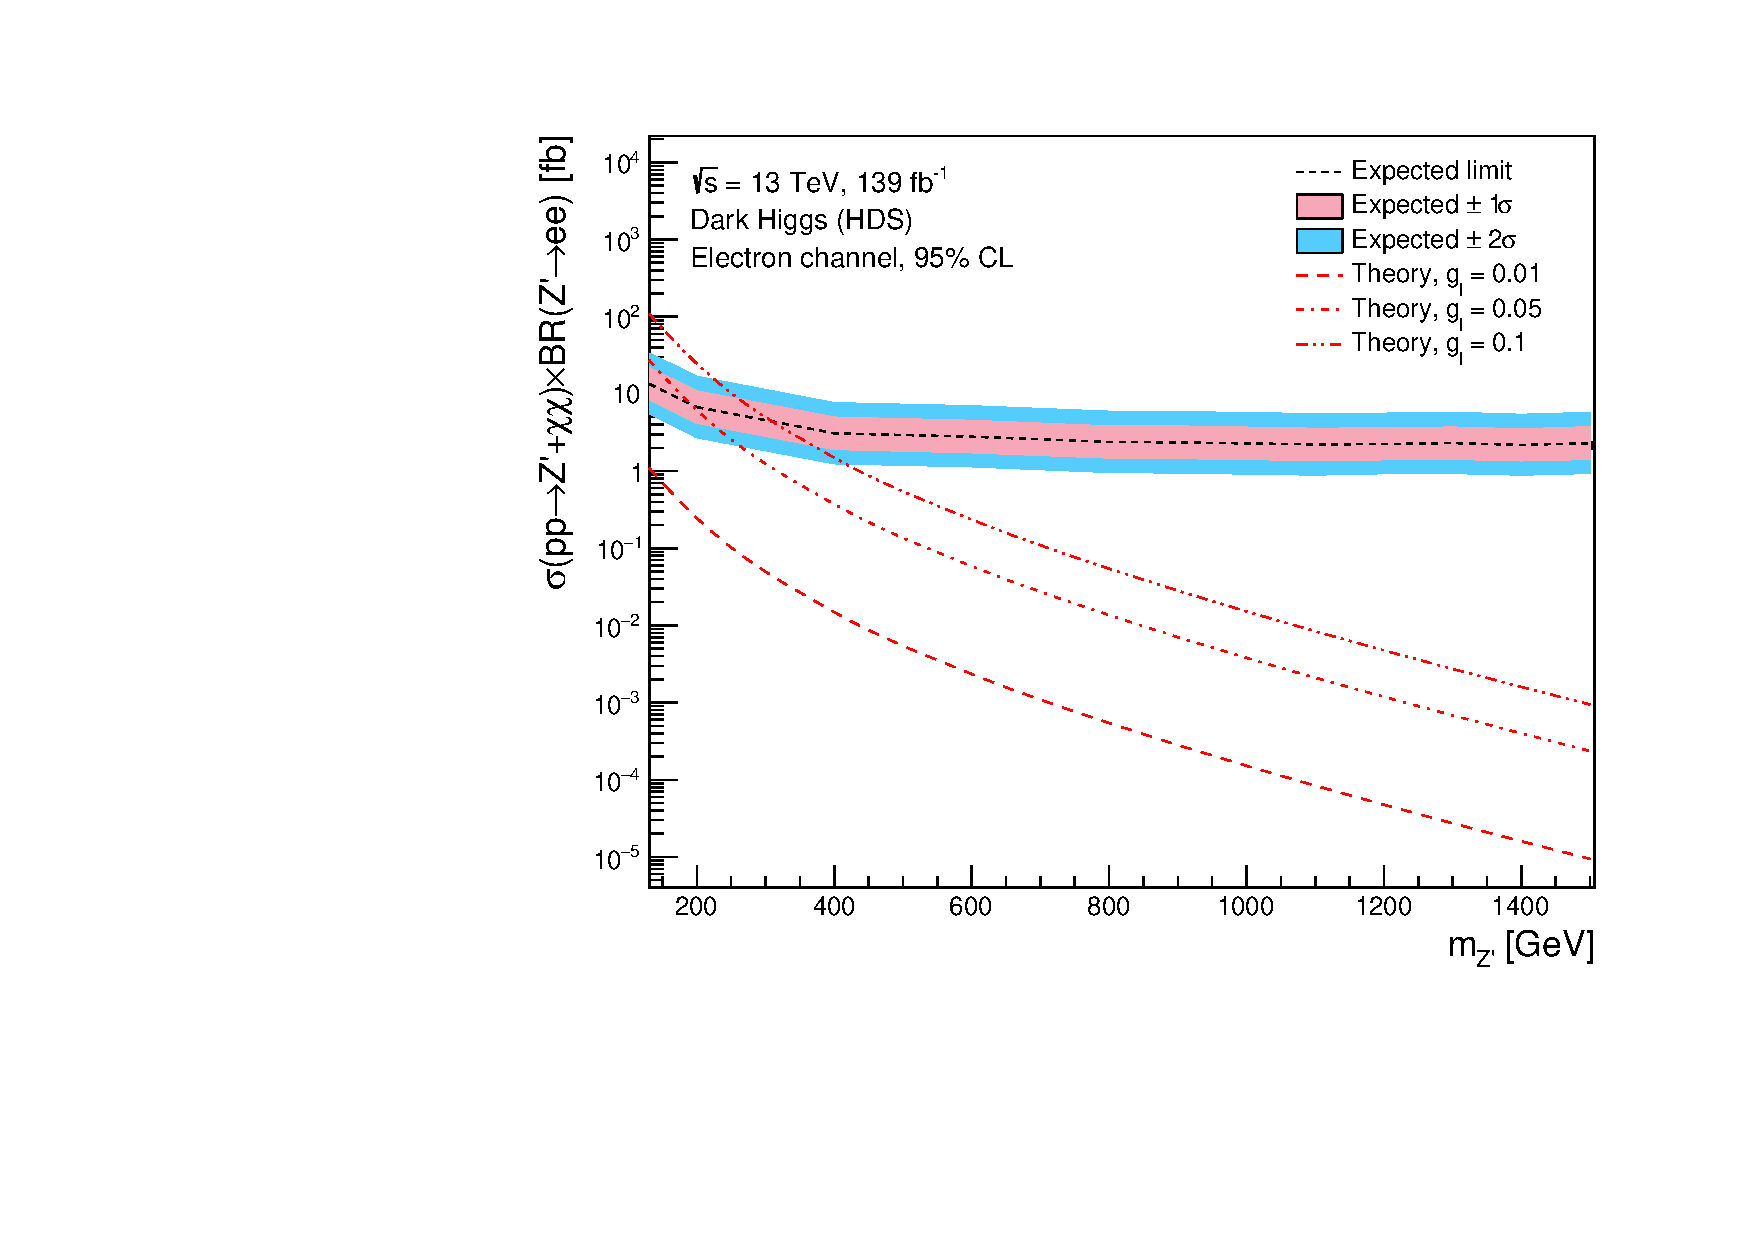
\includegraphics[width=1\textwidth]{Limits/DH_HDS/mass_exclusion_ee.pdf}
      \end{subfigure}
   \hfill
   \begin{subfigure}[b]{0.49\textwidth}
      \centering
      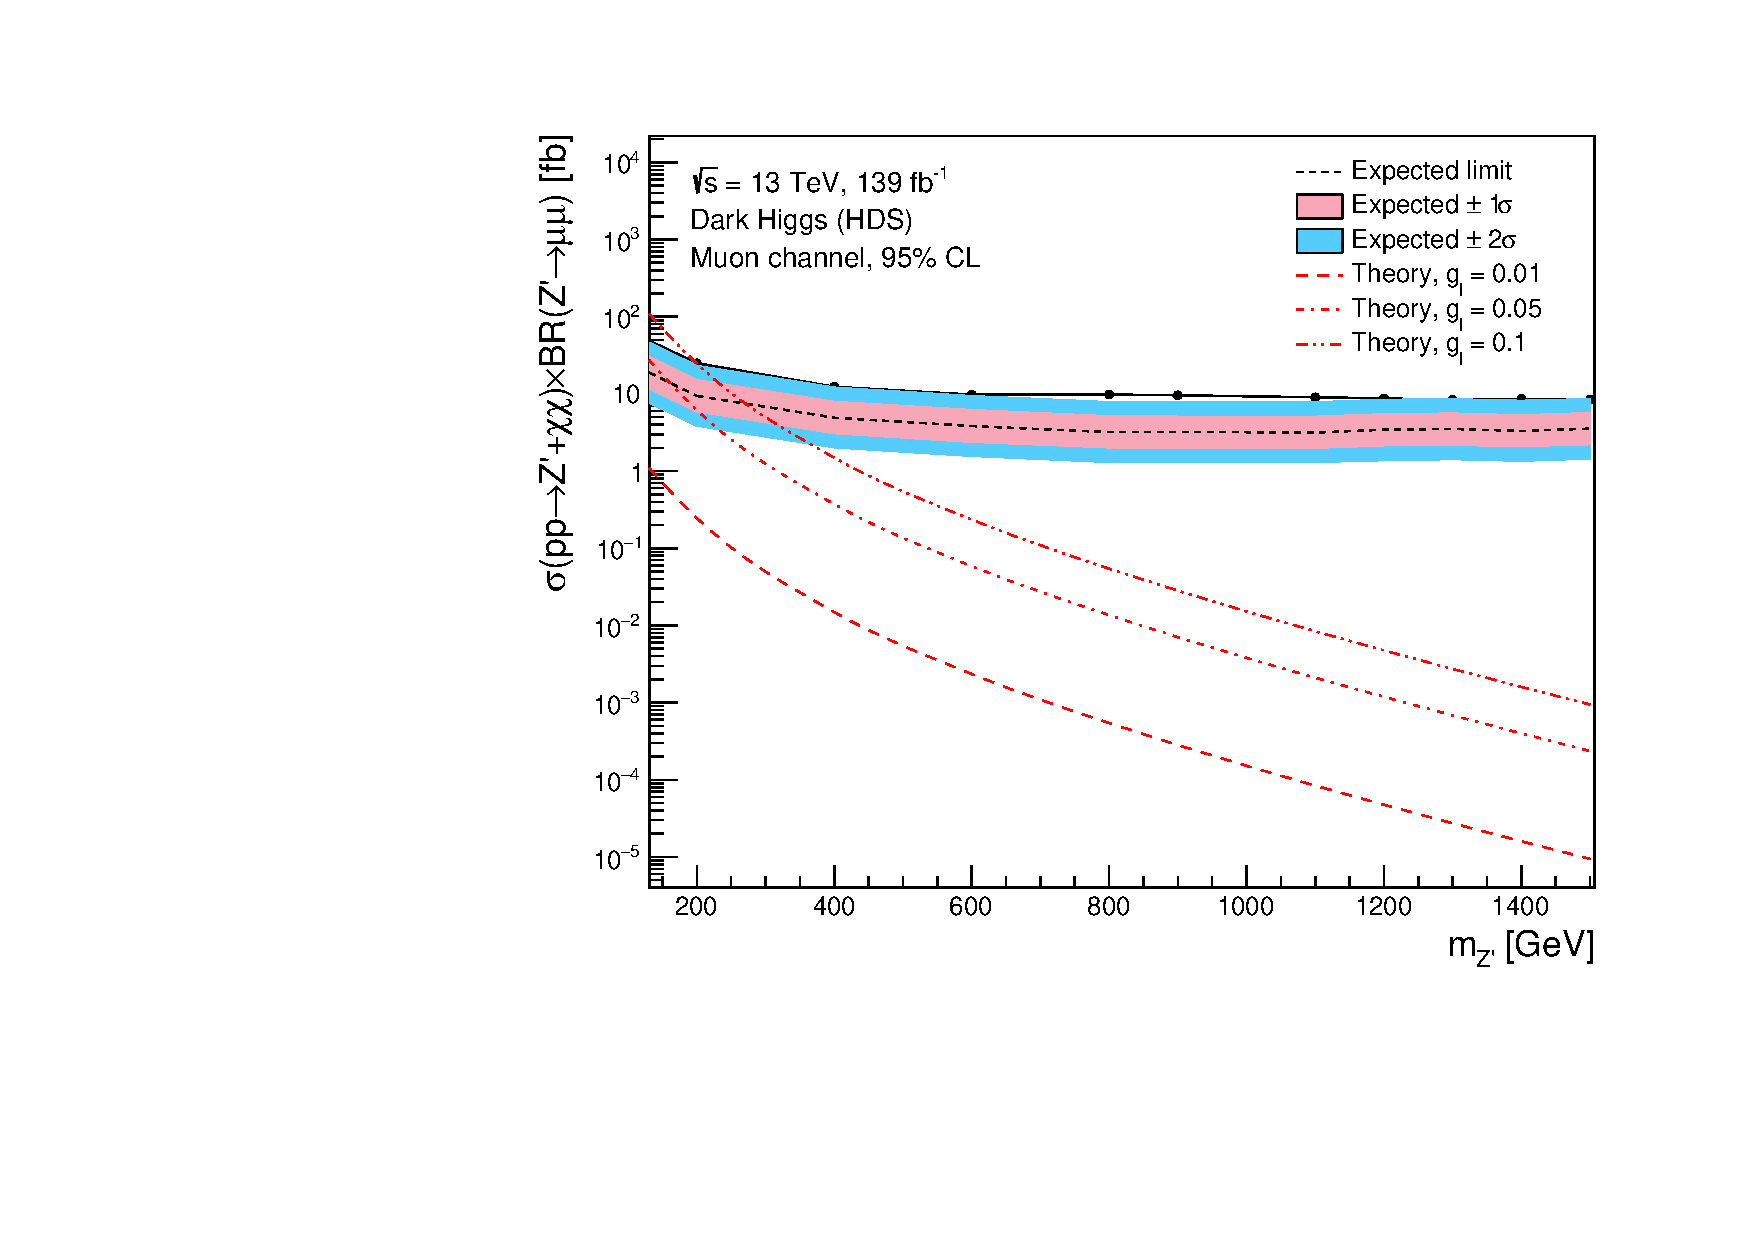
\includegraphics[width=1\textwidth]{Limits/DH_HDS/mass_exclusion_uu.pdf}
      \end{subfigure}
   \caption{Mass exclusion limits of $ee$ and $\mu\mu$ channel for all Z' DH HDS model}\label{fig:DH_HDS_exclusion_ee_uu}
\end{figure}
\noindent We can furthermore statistically combine both of these results to get the exclusion on a general dilepton final state. Following this method for all other five models\footnote{For more plots look at the GitHub repo: in \href{https://github.com/rubenguevara/Master-Thesis/tree/master/Plots/XGBoost/DH_HDS}{https://github.com/rubenguevara/Master-Thesis\\/tree/master/Plots/XGBoost/DH\_HDS} changing "DH\_HDS" for the model of interest} 
we can get the results in Figure \ref{fig:model_dep_exclusions}.\\
\\One thing to note about the mass exclusion limits above, is that as the lepton coupling for all models being tested was chosen to be $g_l=0.01$, we decided to include how the limits would look if we increased this coupling 
to $g_l=0.05$ and $g_l=0.1$. Doing so we have assumed that the efficiency of the cuts stays the same, as well as the number of background events on the last bin. This assumption is noteworthy due to the fact that if we increased the lepton coupling constant of our model, this would increase the branching ratio 
of the leptonic decays. Meaning that when simulating the events we would have gotten more events. As one of the greatest challenges to overcome in this thesis was the imbalanced dataset, this fact would have helped mitigate the problem. 
In addition, a general rule of thumb in ML is that the more statistics one has when training a network, the better the network will learn. The point of this information is that by increasing the lepton coupling constant of the signal, the network 
might have a greater efficiency when learning, as well as reduce the number of background events on the last bin. However, due to time constrains on this thesis we did not have the chance to explore the possibility of simulating more events.
\clearpage
\section{Mass exclusion limits for the combined channels}
\begin{figure}[!ht]
	\centering
	\begin{subfigure}[b]{0.49\textwidth}
      \centering
      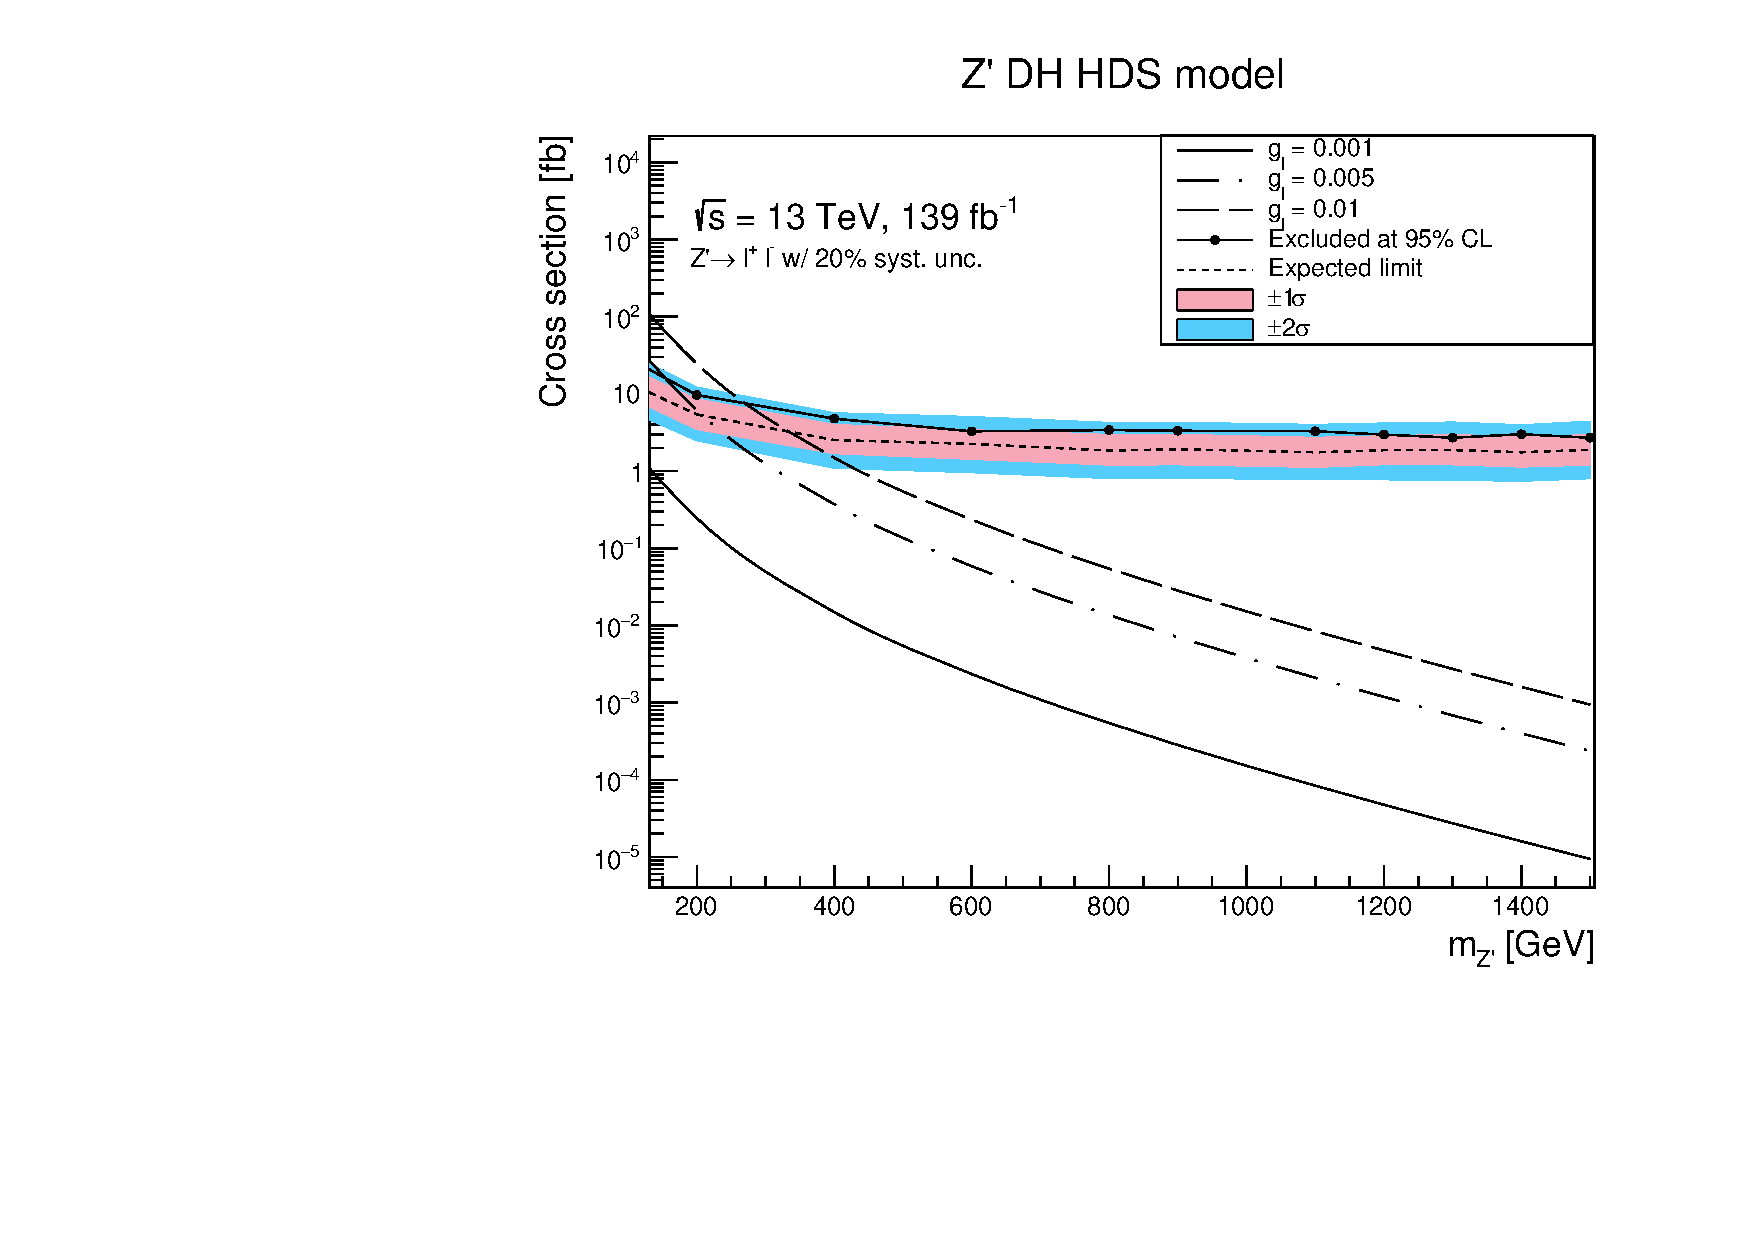
\includegraphics[width=1\textwidth]{Limits/DH_HDS/mass_exclusion_comb.pdf}
   \end{subfigure}
   \hfill
   \begin{subfigure}[b]{0.49\textwidth}
      \centering
      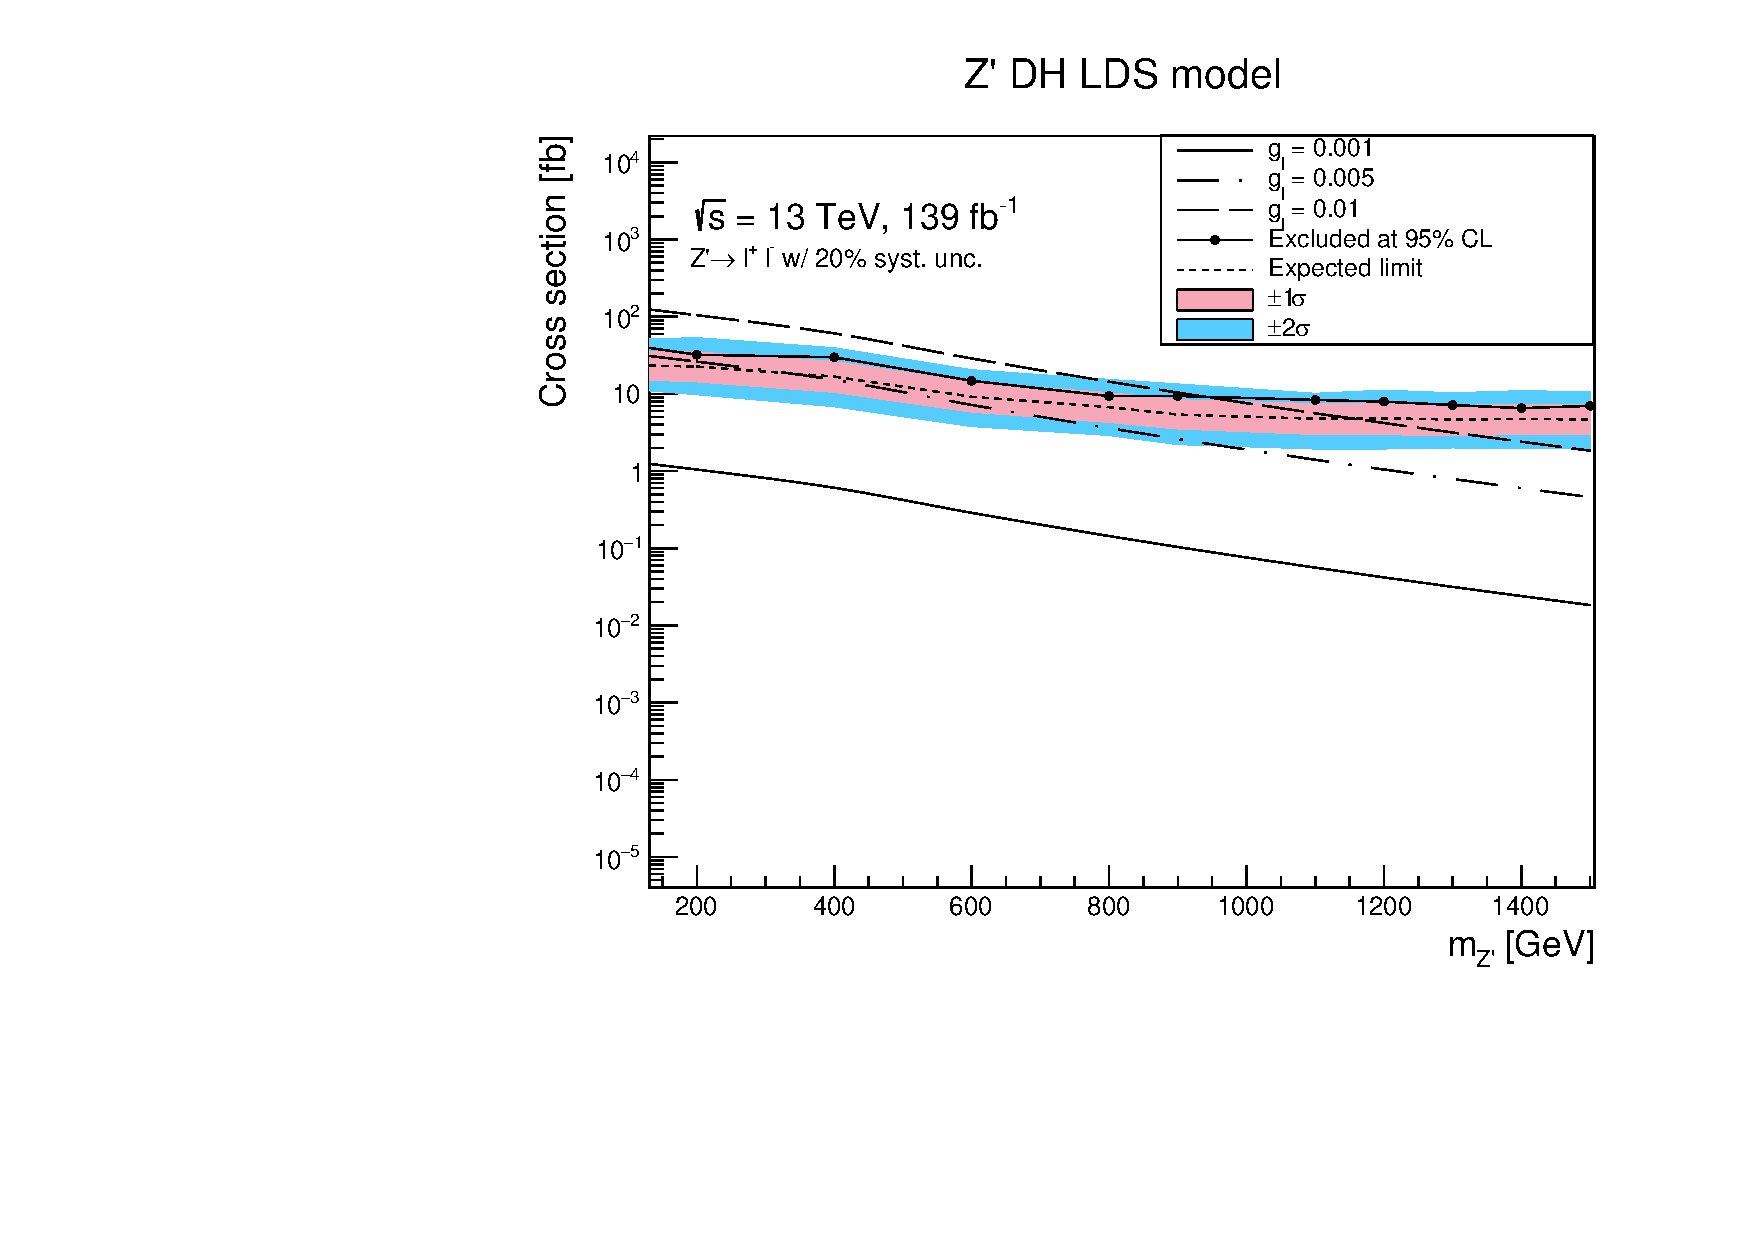
\includegraphics[width=1\textwidth]{Limits/DH_LDS/mass_exclusion_comb.pdf}
   \end{subfigure}
   \hfill
   \begin{subfigure}[b]{0.49\textwidth}
      \centering
      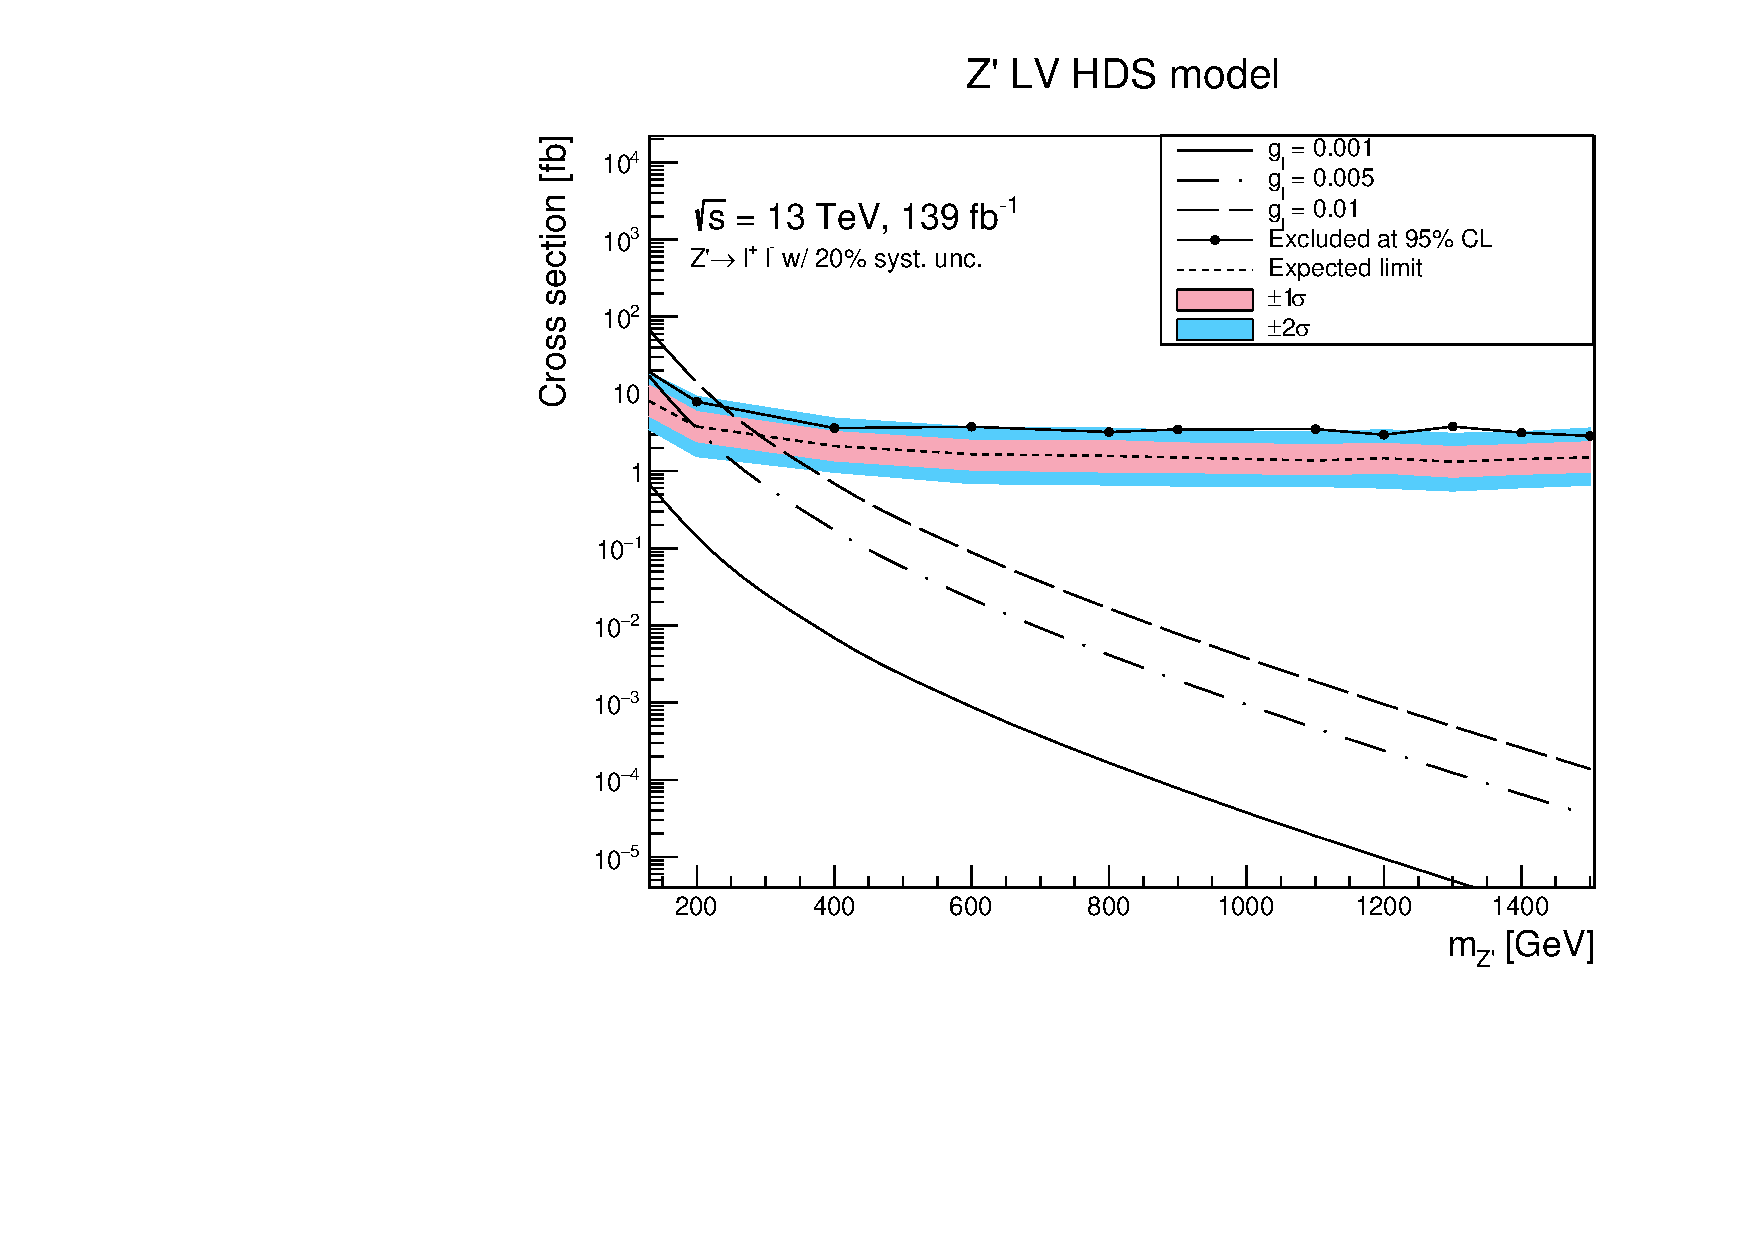
\includegraphics[width=1\textwidth]{Limits/LV_HDS/mass_exclusion_comb.pdf}
   \end{subfigure}
   \hfill
   \begin{subfigure}[b]{0.49\textwidth}
      \centering
      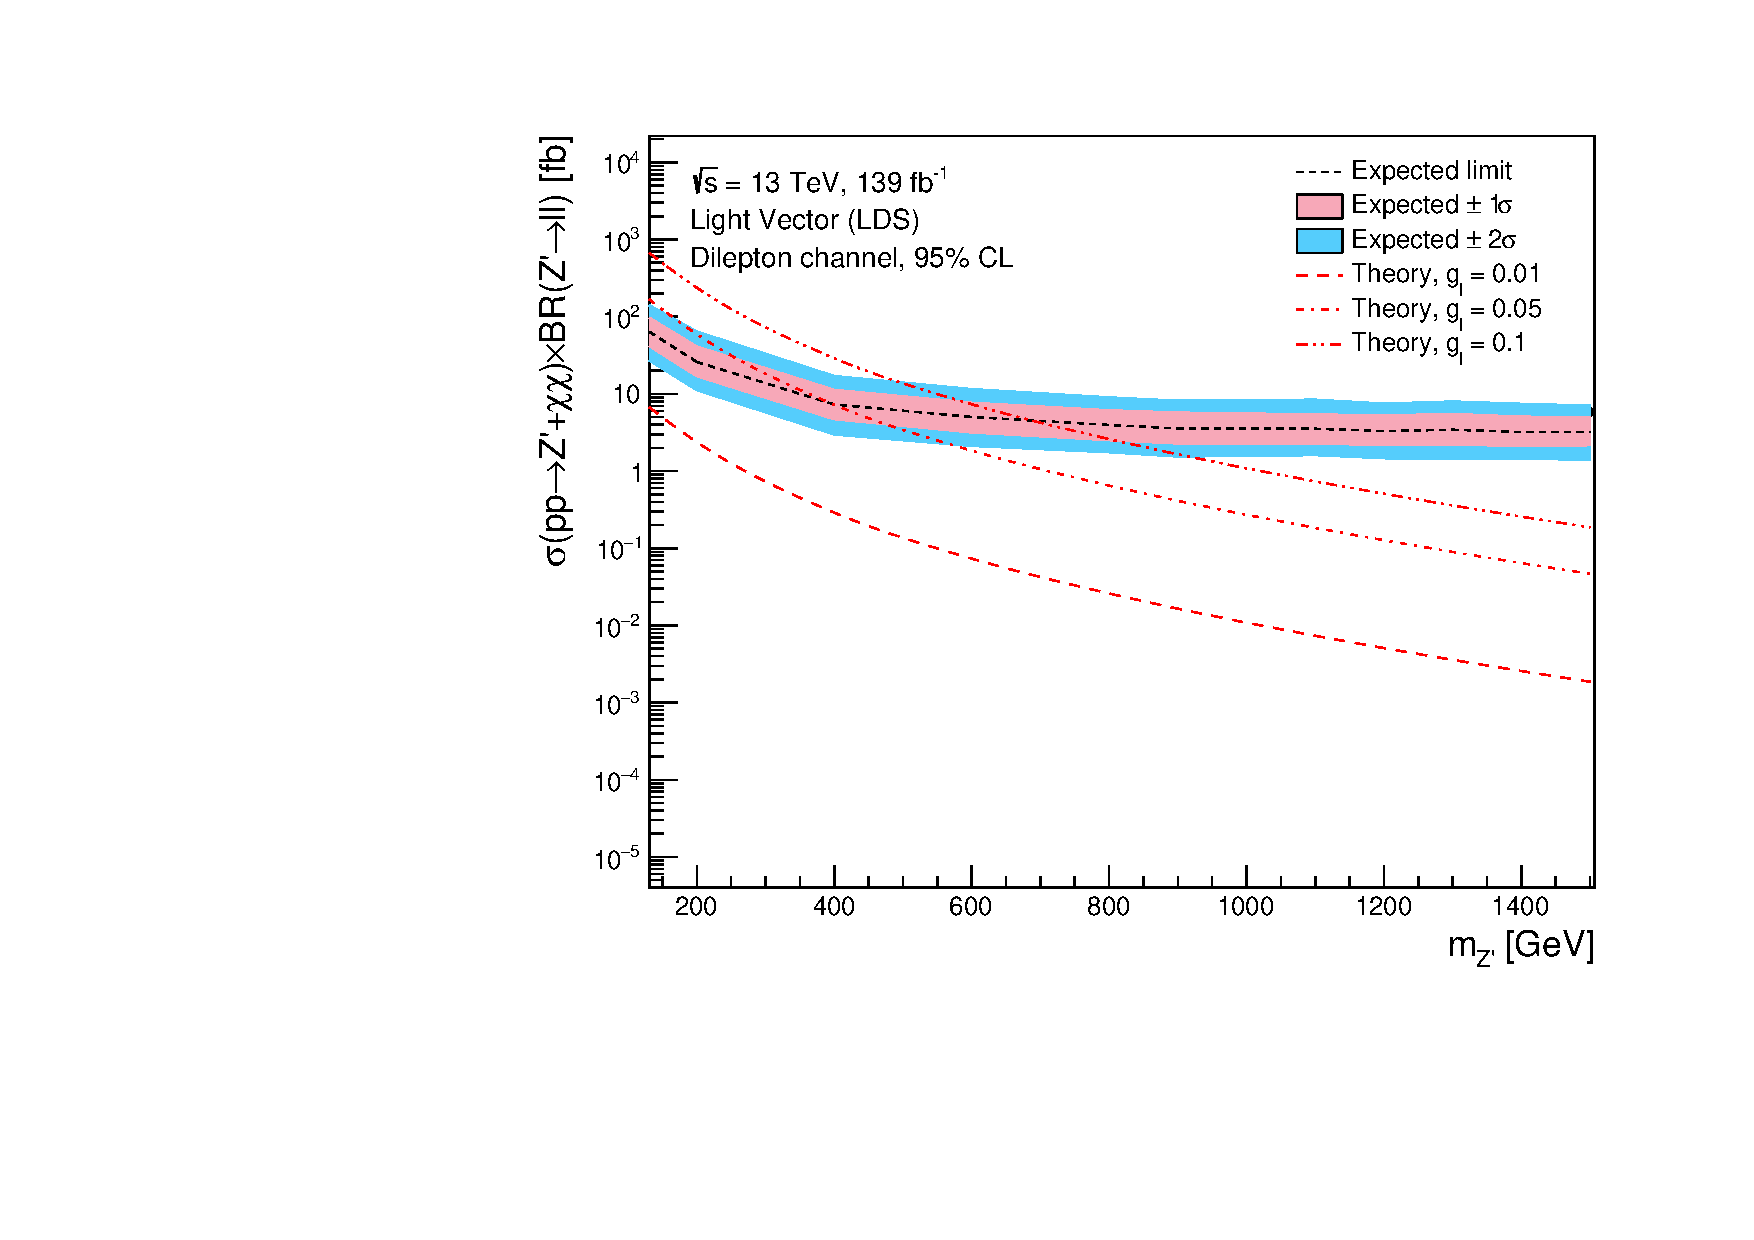
\includegraphics[width=1\textwidth]{Limits/LV_LDS/mass_exclusion_comb.pdf}
   \end{subfigure}
   \hfill
	\begin{subfigure}[b]{0.49\textwidth}
      \centering
      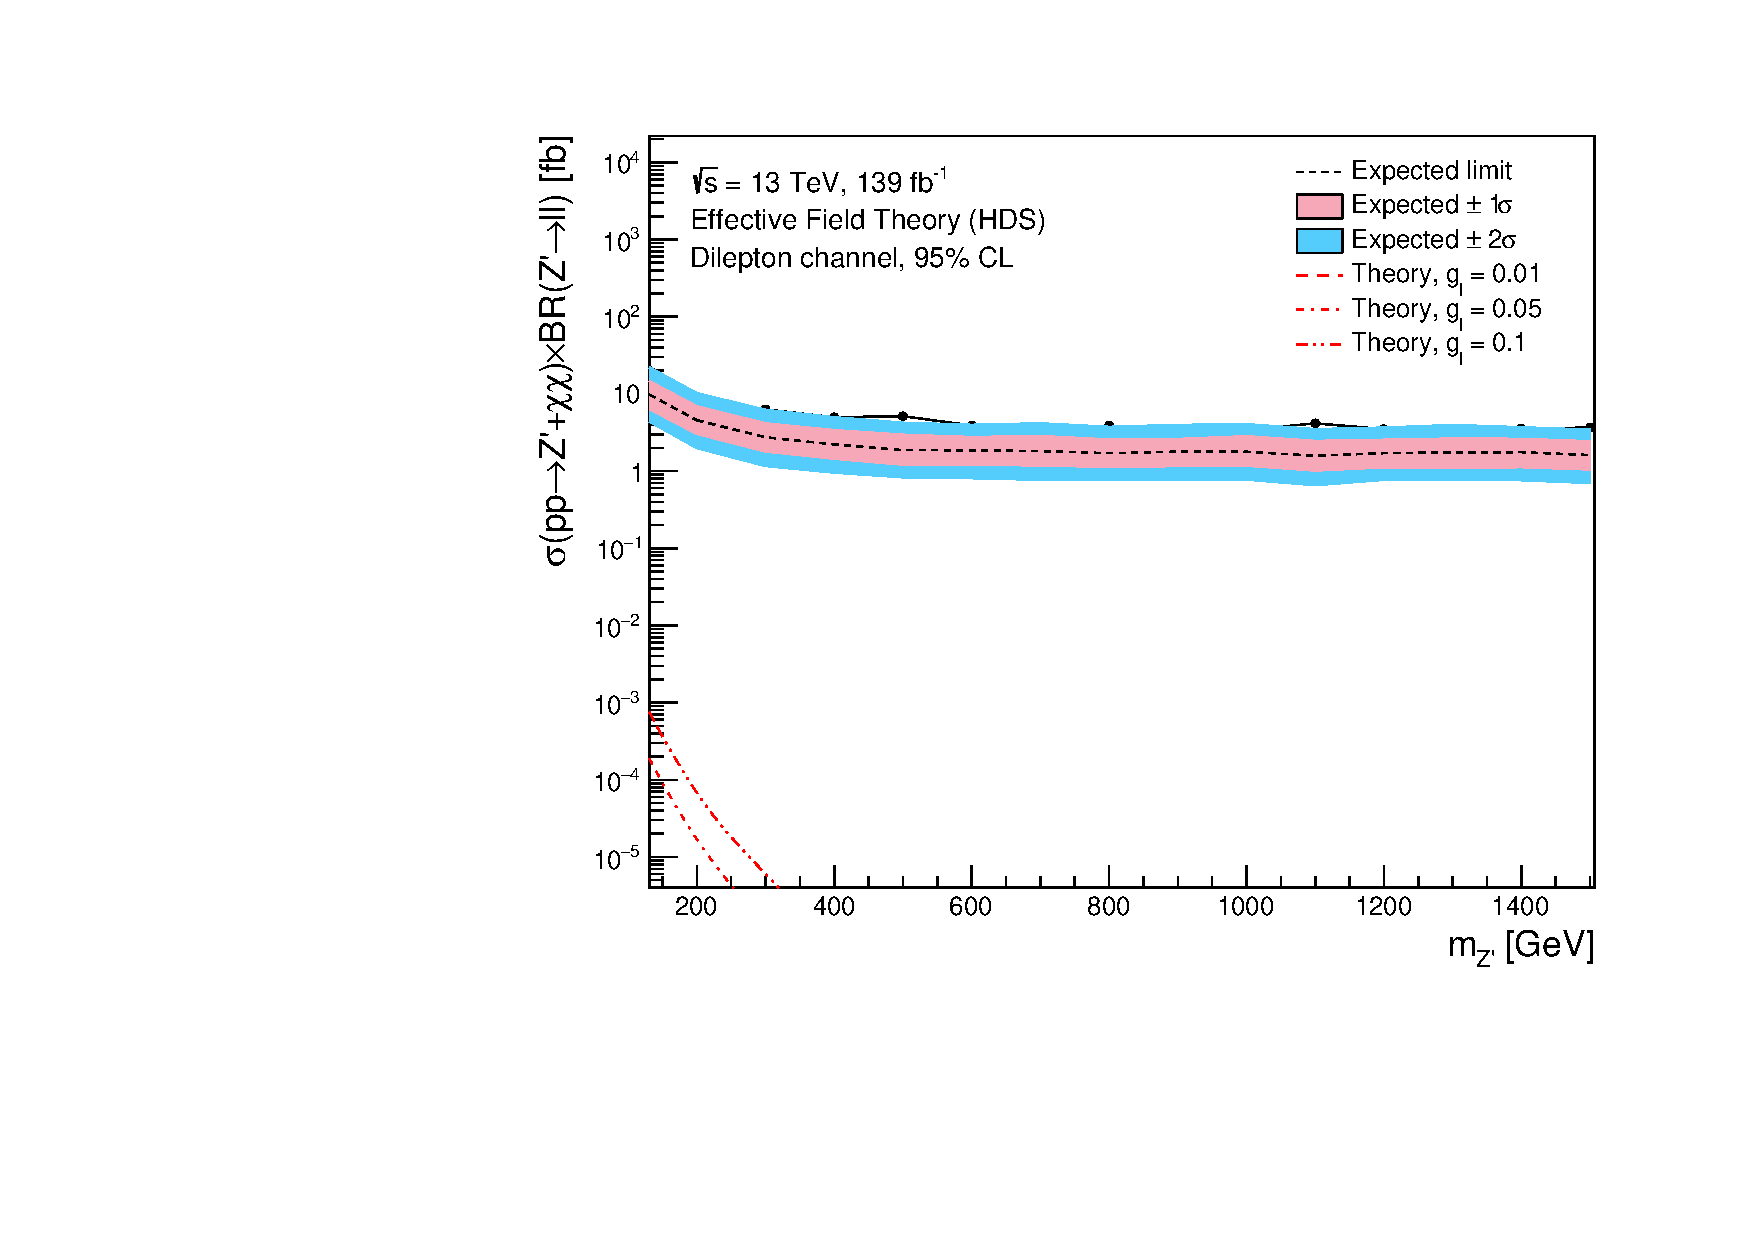
\includegraphics[width=1\textwidth]{Limits/EFT_HDS/mass_exclusion_comb.pdf}
   \end{subfigure}
   \hfill
   \begin{subfigure}[b]{0.49\textwidth}
      \centering
      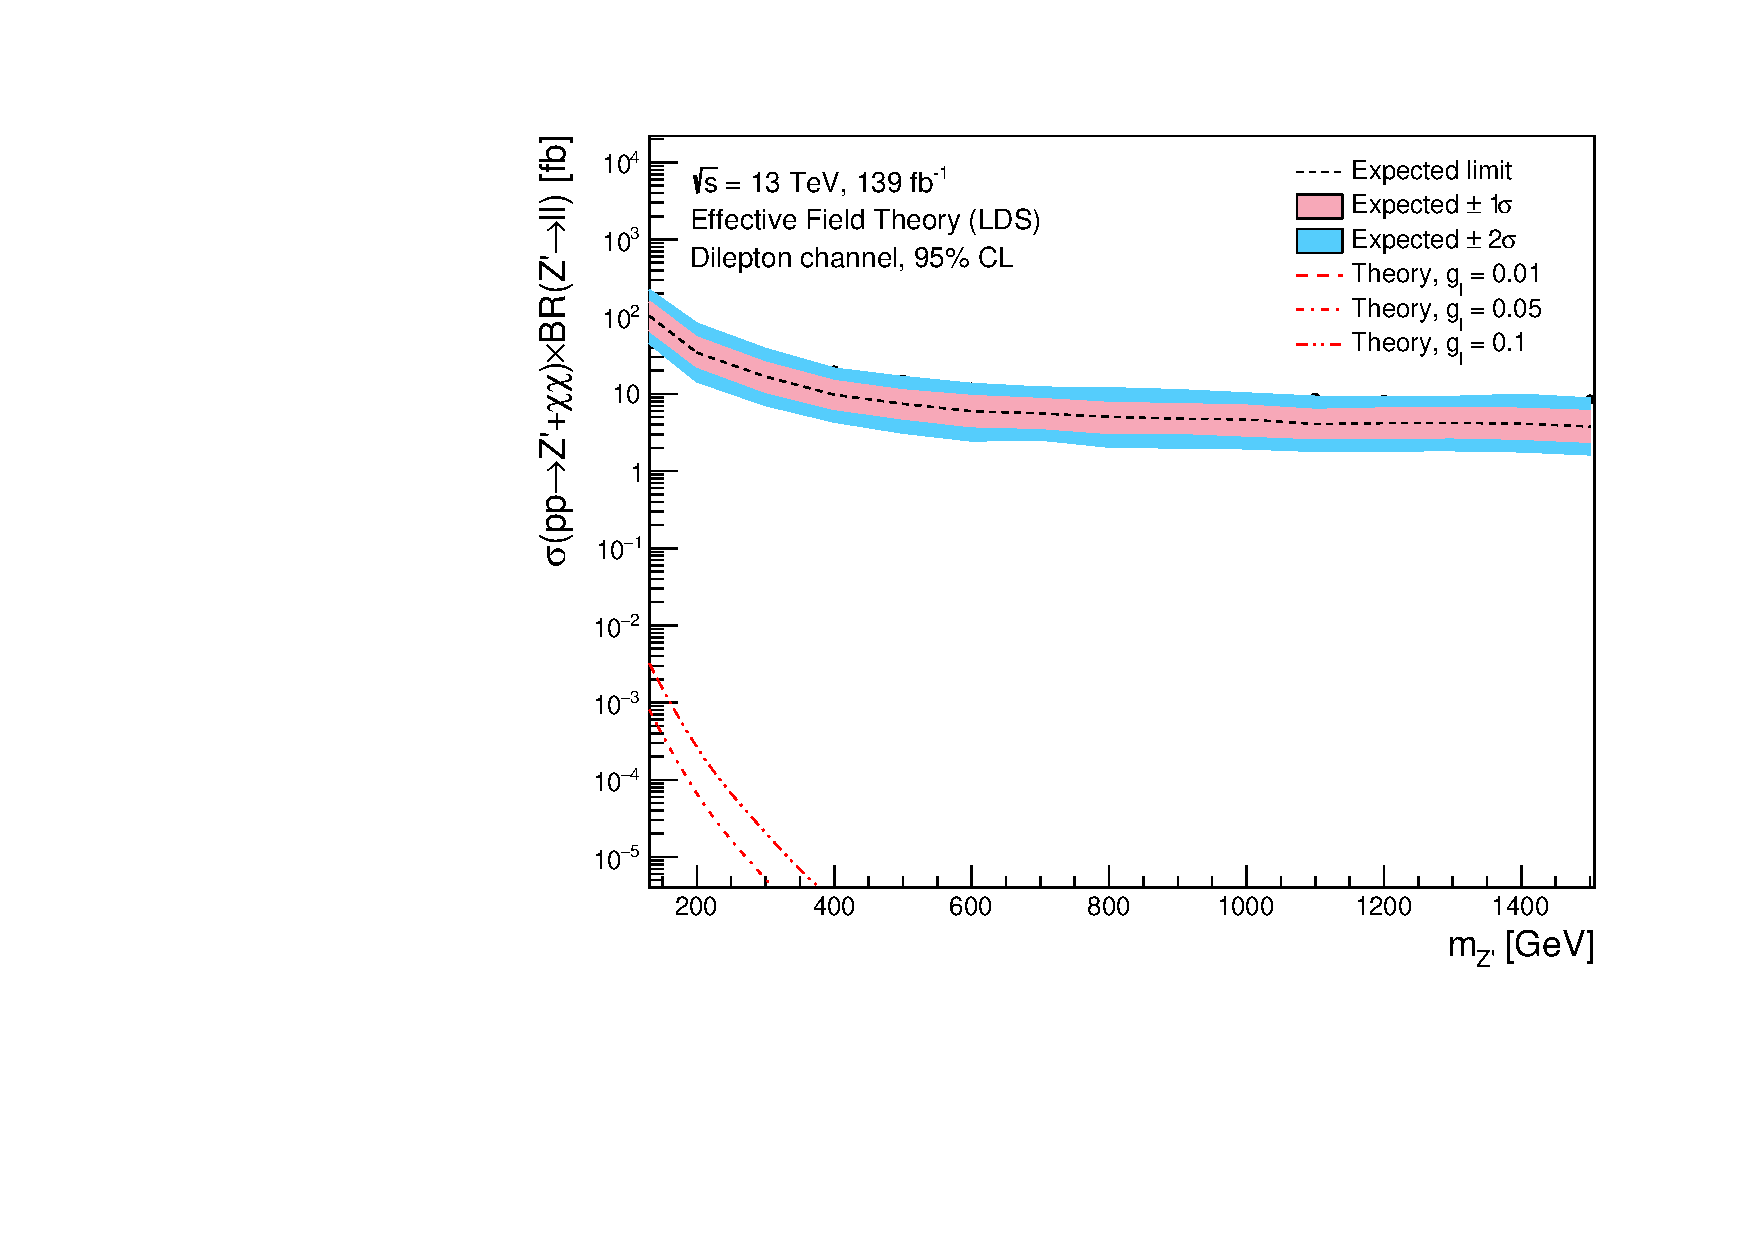
\includegraphics[width=1\textwidth]{Limits/EFT_LDS/mass_exclusion_comb.pdf}
   \end{subfigure}
   \caption[Mass exclusion limits of combined $ee$ and $\mu\mu$ channel for all models]{Mass exclusion limits of combined $ee$ and $\mu\mu$ channel for all models}\label{fig:model_dep_exclusions}
\end{figure}
\clearpage

\end{document}